\documentclass[11pt]{beamer}
\usepackage{color,soul}
\usepackage[utf8]{inputenc}
\usepackage{amsmath}
\usepackage{amsfonts}
\usepackage{amssymb}
\usepackage{algpseudocode} % uses algorithmicx package automatically
\usepackage{mathrsfs}
\usepackage{graphicx}
\usepackage{tikz}
\usepackage{pgfplots}
\begin{document}
\centering
\begin{frame}
\begin{tikzpicture}[scale=0.8]
  %% \begin{axis}
  %% \draw[step=0.5,gray] (-5,-5) grid (5,5);
  \draw[ultra thick,gray] plot[smooth] coordinates {(-6,0)(-5,0)(-3,3) (0,-1) (3,3) (5,0)};
  \node (ox) at (-4,-1) {o(x)};

  \only<2>{
    \path[draw,dotted,blue,very thick] (-5,5) -- (5,5);
  }
  %% \addplot+[ycomb,black,thick] {1};
  %% \node[above] (g1) at (0,4) {};

  \onslide<2->{
    \path[draw,red,thick] (0,-1) -- (0,4) circle (1.5pt);
    \node[above] at (0,4.25) {$g_1+o(x_1)$};
  }
  
  \only<2,3>{
    \path[draw,green,dotted,very thick] (-5,4) -- (5,4);
  }
  
  \onslide<3->{
    \path[draw,red,thick] (-3,3) -- (-3,2) circle (1.5pt);
    \node[below] at (-3,1.5) {$g_2+o(x_2)$};
  }

  \only<3,4,5>{
    \path[draw,dotted,blue,very thick] (-5,3.5) -- (0,3.5);
  }
  
  \onslide<4->{
    \path[draw,red,thick] (3,3) -- (3,4.5) circle (1.5pt);
    \node[below] at (3,5.25) {$g_3+o(x_3)$};
  }
  \only<3->{
    \path[draw,dotted,blue,very thick] (0,5) -- (5,5);
  }
  \only<4->{
    \path[draw,green,dotted,very thick] (-5,4.5) -- (5,4.5);
  }
  %% \end{axis}
\end{tikzpicture}
\end{frame}
\end{document}
